\documentclass[11pt]{article}
%%%%%%%%%%%%%%%%%%%%% Load packages and options
\usepackage{amsmath}
\usepackage{amsfonts}
\usepackage{amsthm}
\usepackage{mathrsfs}
\usepackage{enumerate}
\usepackage{blkarray}
\usepackage[dvipsnames]{xcolor}
\usepackage[T1]{fontenc}
%\usepackage{listings}
\usepackage{matlab-prettifier}
\lstset{
  style             = Matlab-editor,
  basicstyle        = {\mlttfamily\color{ForestGreen}},
  escapechar        = \#,
  mlshowsectionrules = true,
  upquote           = true
}
\newcommand\ph\mlplaceholder

\usepackage{graphicx}
%\usepackage{hyperref}   % to include web-links in your pdf document
\usepackage{verbatim}

%%%%%%%%%%%%%%%%%%% Set margins and basic spacing
\textwidth=6.6in
\textheight=9.8in
\oddsidemargin -0.3in
\topmargin -0.7in
\parindent 0in
\parskip 0.3cm

%%%%%%%%%%%%%%%%%%  Define some useful shortcuts for parentheses that scale
\newcommand{\p}[1]{\left( {#1} \right)}
\newcommand{\s}[1]{\left[ {#1} \right]}

%\renewcommand{\baselinestretch}{1.1}    % for double spacing use 2.0 (or 1.5)
%%%%%%%%%%%%%%%%%%%%%%%%%%%%%%%%%%%%%%%%%%%%%%%%%%%%%%%%%%%%%%%%%%%%%%%%%%%%%%%%%
%%%%%%%%%%%%%%%%    BEGIN DOCUMENT
%%%%%%%%%%%%%%%%%%%%%%%%%%%%%%%%%%%%%%%%%%%%%%%%%%%%%%%%%%%%%%%%%%%%%%%%%%%%%%%%%
\begin{document}
\pagestyle{empty}    % style "plain" gives page numbers at the bottom

\Large
{\bf Geog 331 \hfill Colgate University}
\normalsize
\centerline{\bf Activity 7}
\centerline{\bf by Kayla Logar}   % FIXME

%\includegraphics[width=2.5in]{cobweb2_r2_9.jpg}
%\includegraphics[width=2.5in]{profile_r2_9.jpg}

\section{Describe the differences in reflected/emitted light across the land surface. What are some major differences that you notice in the different landcover classes?
}  % The  makes it so the section number doesn't appear.
We see several different patterns in reflected/emitted light across the land surface, including that the algae tends to reflect more light than the remaining water surface, which enables us to denote this difference. Furthermore, these areas both reflect much less light than the surrounding land area. Of the landcover classes, forests appear to reflect the least light, with forest area appearing the darkest shade of pink in the figure. The agriculture and wetlands areas are a lighter shade of pink and therefore reflect a little more light, followed by the built areas, which appear to be some of the lightest regions in the map, indicating that they reflect the most light.


\section{What land classes have the highest rates of misclassification? What sort of bias would this introduce if you used these predictions in an analysis?}

We see the highest rates of misclassification in areas of agriculture and built. Of the 60 areas of agriculture, 10 are misclassified (5 as built and 5 as wetlands) for a misclassification rate of approximately 16.7\%. Of the 55 areas of built land, 4 are misclassified for a misclassification rate of approximately 7.3\%. Likewise, approximately 3.3\% of forest areas are misclassified and approximately 1.7\% of wetlands areas are misclassified. On the other hand, we see that algal bloom and open water are classified very accurately, with all 60 areas of each being correctly classified. So, all of the misclassifications occur on areas of land, not water.

Overall, if we consider these areas and lapses of accuracy, an analysis using these predictions would involve the bias that comes as a result of underrepresenting areas of agriculture and built areas.

\section{Show both maps from your classification outcome in your document and include confusion matrices. Describe the spatial patterns and general location of the different landcover classes. Describe the general differences between predictions from each method.}

\begin{center}
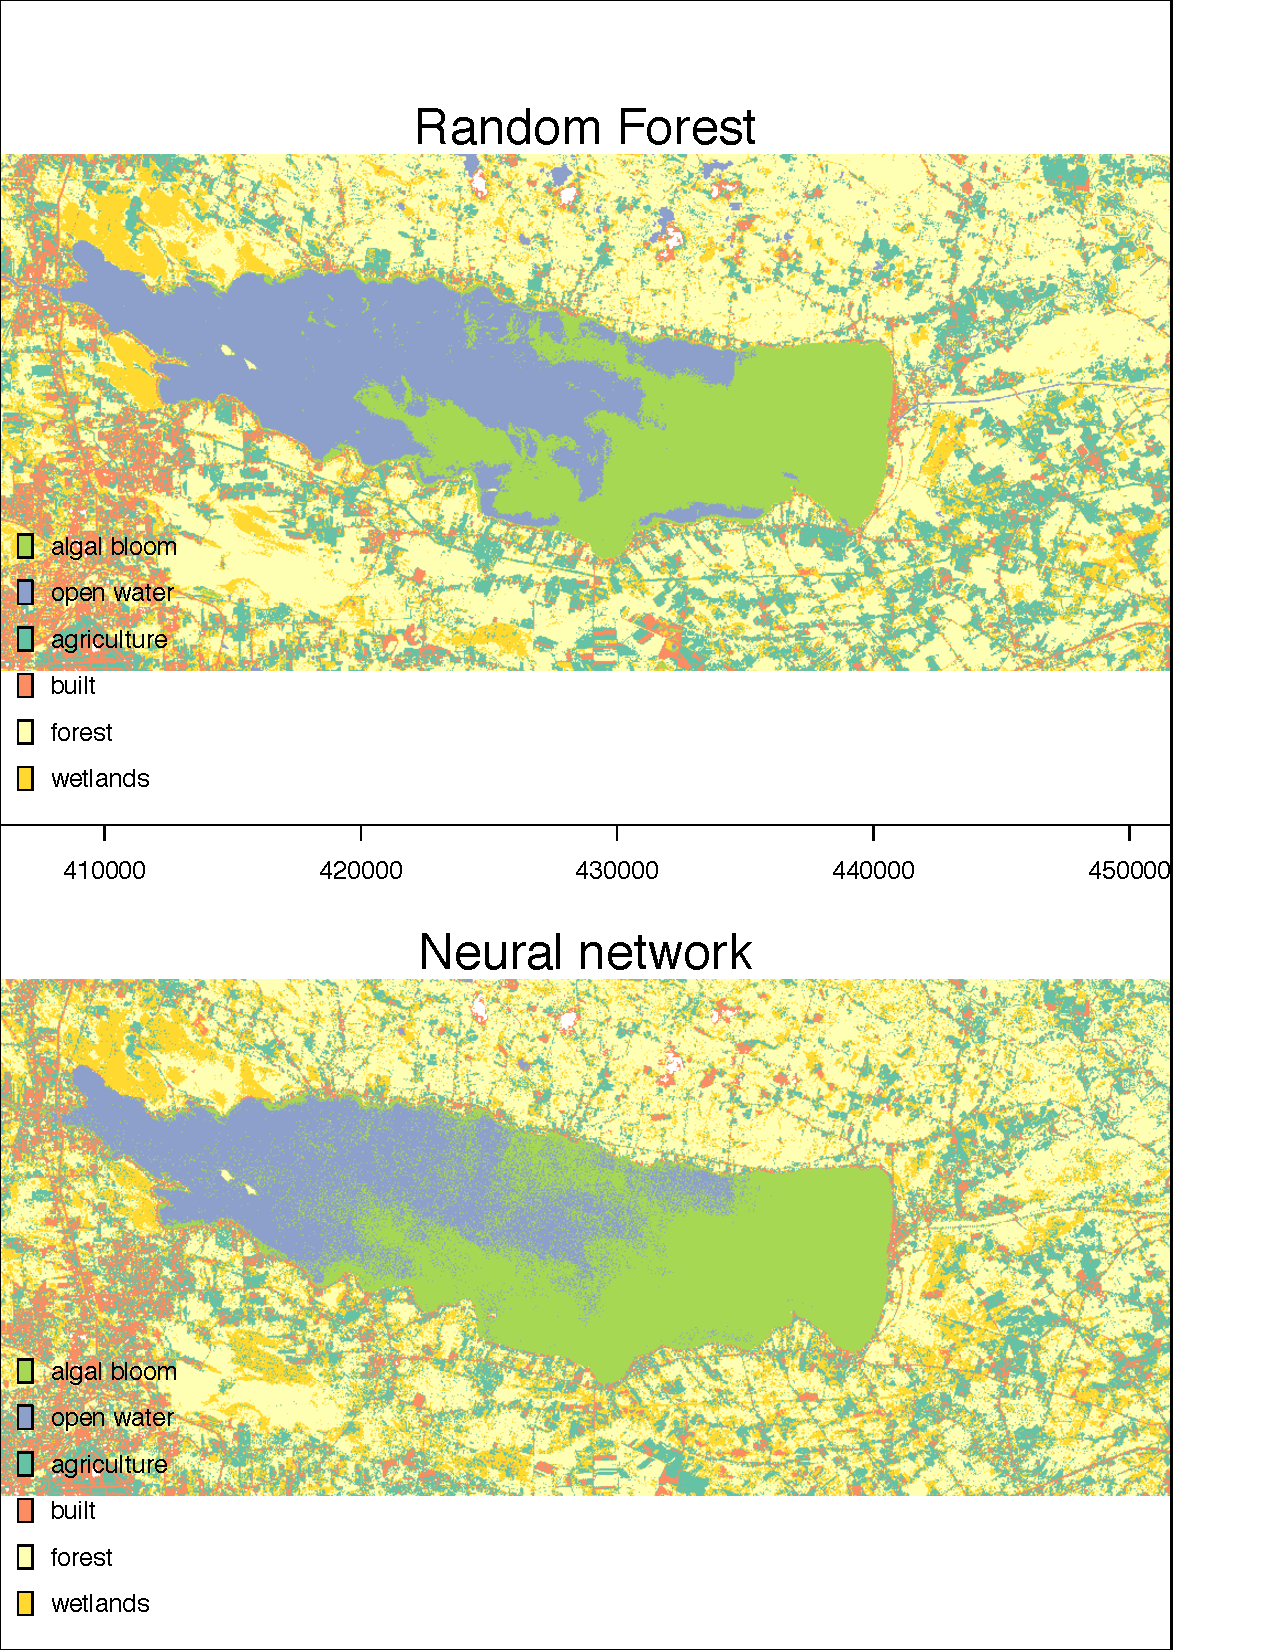
\includegraphics[width = 5in]{plots.pdf}
\end{center}

\subsection*{Confusion matrices}
\[
\begin{blockarray}{lcccccc}
& & & Random Forest & & & \\
& & & Reference & & & \\
Prediction & algal bloom & open water & agriculture & built & forest & wetlands\\
\begin{block}{l(cccccc)}
algal bloom & 60 & 0 & 0 & 1 & 0 & 0 \\
open water & 0 & 60 & 0 & 0 & 0 & 0 \\
agriculture & 0 & 0 & 50 & 3 & 0 & 0  \\
built & 0 & 0 & 5 & 51 & 0 & 0  \\
forest & 0 & 0 & 0 & 0 & 58 & 1 \\
wetlands & 0 & 0 & 5 & 0 & 2 & 59 \\
\end{block}
\end{blockarray}
 \]
 
 \[
\begin{blockarray}{lcccccc}
& & & Neural Networks & & & \\
& & & Reference & & & \\
Prediction & algal bloom & open water & agriculture & built & forest & wetlands\\
\begin{block}{l(cccccc)}
algal bloom & 60 & 1 & 0 & 0 & 0 & 0 \\
open water & 0 & 59 & 0 & 0 & 0 & 0 \\
agriculture & 0 & 0 & 34 & 5 & 0 & 2  \\
built & 0 & 0 & 8 & 47 & 0 & 0  \\
forest & 0 & 0 & 3 & 3 & 44 & 1 \\
wetlands & 0 & 0 & 15 & 0 & 16 & 57 \\
\end{block}
\end{blockarray}
 \]

Based on the maps and confusion matrices above, we see that the neural networks prediction technique features less agriculture and built areas. This reflects the difficulties of predicting agriculture using neural networks, as described in the activity description. Furthermore, there is a greater area of algae predicted using the neural network model, although the area of algae predicted is less dense and more spotted than in the random forest prediction model.

\section{Knowing each cell is 20 m x 20 m, what is the difference in area predicted to be algal blooms in each method? Which method predicts a higher area of algal bloom?}

In our prediction models, 120,545,200 m$^2$ are predicted to be algal blooms using the neural networks prediction method while 97,492,400 m$^2$ are predicted to be algal blooms using the random forest prediction method. Thus, the difference in area predicted to be algal blooms in each method is 23,052,800 m$^2$, with neural networks predicting a higher area of algal bloom.

\section{Create a raster that shows whether neural network and random forest predictions agree or disagree. Describe the spatial patterns you observe. Where are these areas prone to disagreement between predictions?}

In the raster plot below, we see the areas with no difference depicted in white and the areas with the most difference between the two prediction methods in green. In this plot, we see that the large area of algal bloom along the right side (most likely eastern side) of the body of water. Though, notably, even the differences in the middle of the water are scattered and mild. Additionally, there are large areas of agreement on the far left of the body of water and scattered throughout the land, particularly in areas of forest - this is most apparent in a large white area on the bottom left that corresponds with an area of forest. Throughout the plot, we see that the areas of forest tend to have somewhat lower differences which are more likely to be represented with the more pinkish color representing lower differences. The largest differences appear in the green areas - some of the largest of which occur towards the top of the map, where the random forest method predicts open water areas while the neural network method predicts wetlands in these same regions.

\begin{center}
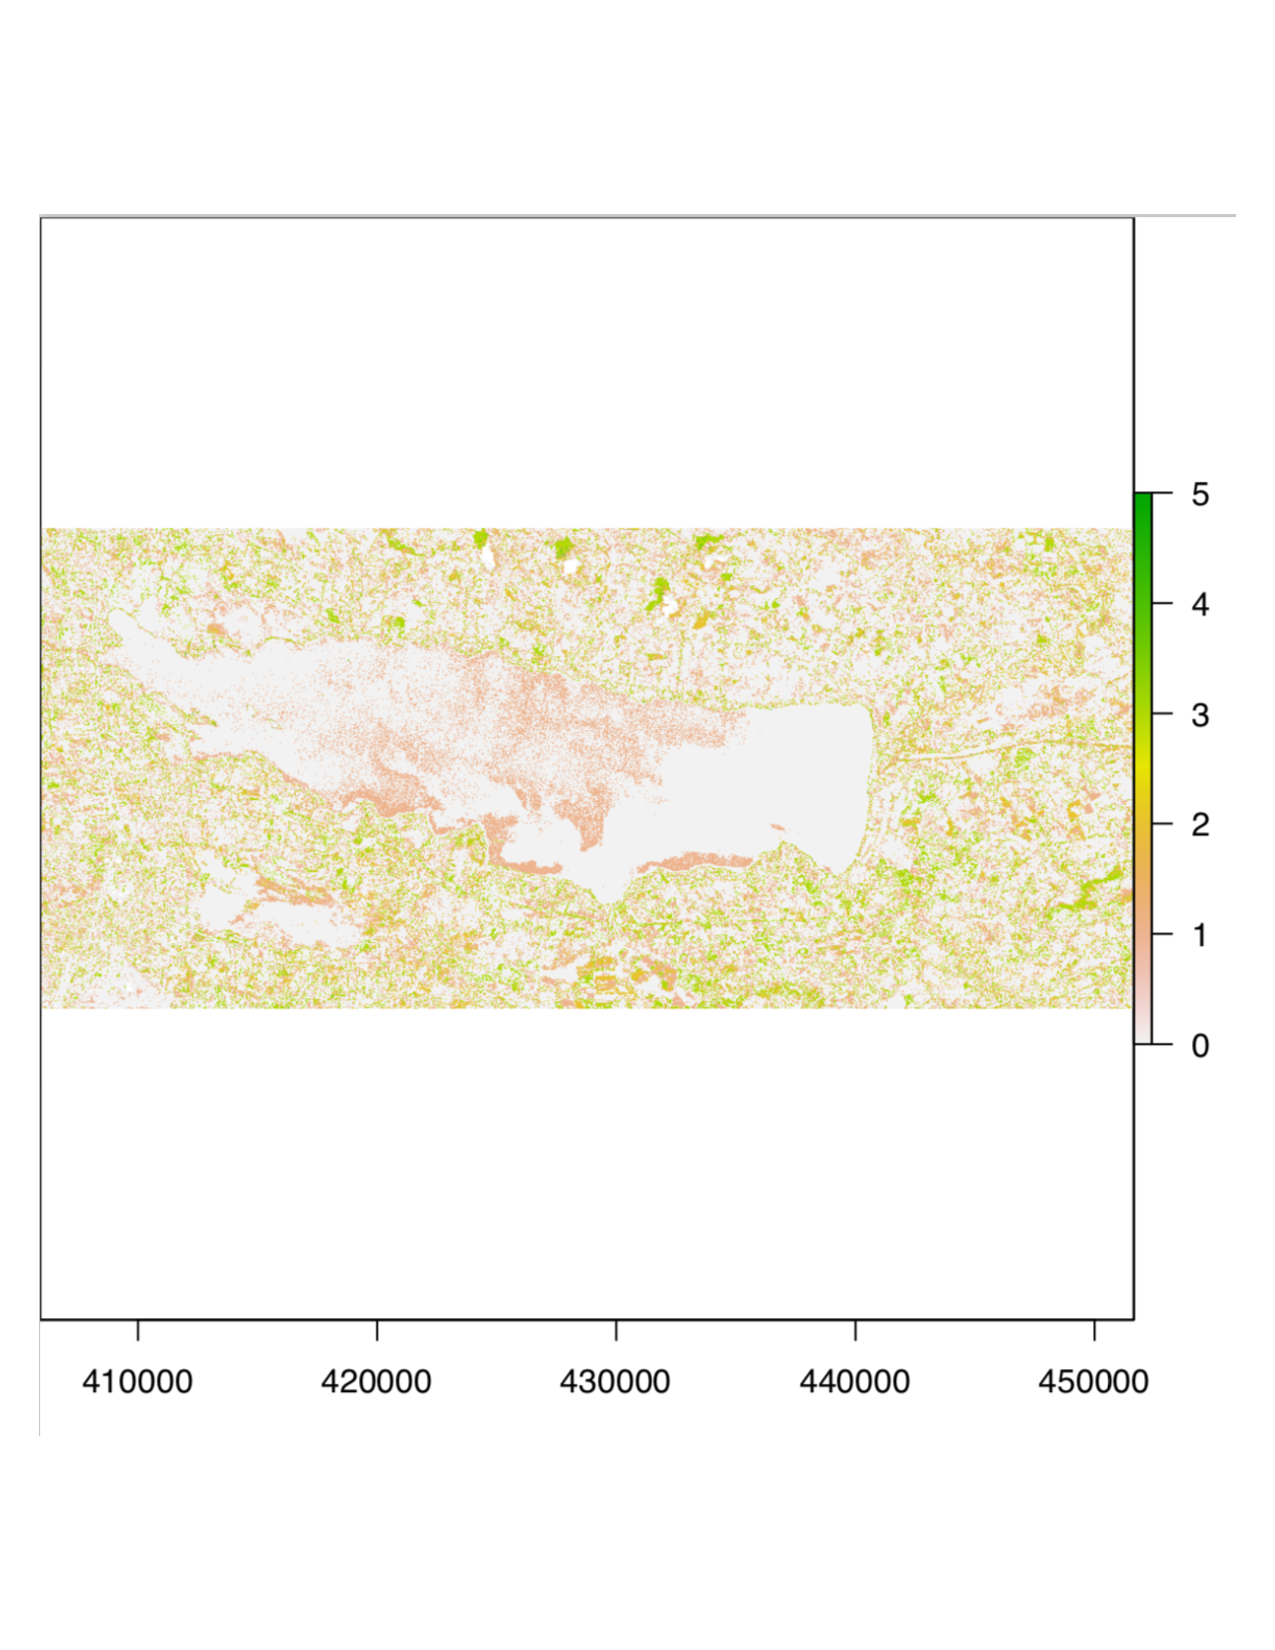
\includegraphics[width=5in]{differenceplot.pdf}
\end{center}

\section{What is the producers and users accuracy for algal blooms for both methods? What is the producers and users accuracy for agriculture for both methods?}

According to the confusion matrices above, we see that the producers' accuracy for algal blooms using both neural networks and random forests is 60/60 = 100\%. Likewise, the users' accuracy for both methods is 60/61 = 98.4\%.

Furthermore, when we consider agriculture, we find a producers accuracy of 34/60 = 56.7\% using neural networks and 50/60 = 83.3\% using the random forest method. For agriculture, we find a users accuracy of 34/41 = 82.9\% using neural networks and 50/53 = 94.3\% using random forests.

\section{Algal blooms are prone to occur in areas where sunlight, stagnant water, and excess nutrient inputs can promote growth. Visually, do you think the landcover around the lake contributes to the algal blooms? Explain your answer. How would you answer this question quantitatively using spatial analysis techniques?}

Yes, based on the landcover around the lake, we see that algal areas more commonly occur around agriculture. This is due to the fact that there are excess nutrient inputs in the form of fertilizer runoff near areas of agriculture. We see that the majority of the algal bloom area occurs near the agricultural area that is right alongside the water at the bottom right (potentially southeast) corner of the body of water. Similarly, some runoff may be coming from the built area that is seen along the right side of the body of water that is also touching the water in the region of large algal bloom. This is plausible because people can produce other forms of nutrient runoff in more developed areas. On the other hand, areas with less algal blooms in the water generally tend to be surrounded by landcover of forest and wetlands, which would release less excess nutrient inputs.

In order to answer this question quantitatively with spatial analysis techniques, I would analyze what landcover types occur along water and how this correlates to the presence of algae in the water alongside a given area of land based on what type of landcover is present.

\section{Which prediction method would you use for a more formal quantitative analysis of question 7? What bias would you need to consider in the interpretation of your results?}

I would use the random forest method to perform a more formal quantitative analysis of question 7 because the random forest method is significantly more accurate than the neural networks method at predicting areas of agriculture, and based on our observations, areas of agriculture may be important to our understanding of algal blooms. Thus, it is important for us to maximize our ability to accurately predict and analyze data regarding areas of agriculture. However, in the interpretation of our results using the random forest method, it is important to note that the producers accuracy using the random forest technique for areas of agriculture is still only around 83.3\%, which is still imperfect, so it will be important to note the limitations of our results. 

\section{This type of prediction can only classify algal growth from a satellite measurement. What might be some of the issues with relying on satellites to observe the presence of algal blooms? What data and approaches might you use to predict whether an algal bloom is expected to occur in the future?}

Given that this type of prediction relies on satellite measurements, there may be issues with the spatial resolution - since algal blooms may start with very small areas, they would likely not be picked up in the beginning until they reached a large enough area to be detected from a satellite. This would then impair our ability to note small areas of algal blooms that would grow into future areas of algal blooms, which would be helpful in the prediction process. In order to predict whether an algal bloom is expected to occur in the future, I might use a few different methods, including using the results of what areas are around the areas of worst algal bloom to note trends that may indicate which areas are most likely to potentially lead to algal bloom, looking at the spread and growth of areas of algal bloom over time, and measuring the nutrients entering the water from the surrounding land areas to note areas of excess nutrients which are likely to lead to algal bloom.

\section{Copy and paste the link to your GitHub code.}



\end{document}
%%%%%%%%%%%%%%%%%%%%%%%%%%%%%%%%%%%%%
%%%%%%%   END DOCUMENT
%%%%%%%%%%%%%%%%%%%%%%%%%%%%%%%%%%%%%

After the end of the document, nothing gets processed, so you can keep
convenient Latex idioms to copy and paste when you need them.

%%%%%%%%%%%%%%%% itemize (bullet list)
\begin{itemize}
\item
\item[a)]
\end{itemize}

%%%%%%%%%%%%%%%% enumerate (numbered list)
\begin{enumerate}
\item
\item[a)]
\end{enumerate}

%%%%%%%%%%%%%%%% aligned equations
\begin{align*}
   &  \\
   &
\end{align*}
% for example
\begin{align*}
   x &= 3  \\
   y &= 4
\end{align*}

%%%%%%%%%%%%%%%% Matlab code
\lstinline|%code in a paragraph|
\lstinputlisting{filename.m}
\begin{lstlisting}
function d=dim1d(xvalues,edges)
% 
end
\end{lstlisting}

%%%%%%%%%%%%%%%% figures
\begin{center}
\includegraphics[width=3in]{file}
\end{center}

%%%%%%%%%%%%%%%% move vertically or horizontally
\vspace{.2in}
\hspace{-.8cm} {\bf Page , Exercises:}
